% (C) Marc Lijour, 2016-2017 
% Licensed under a Creative Commons License BY-SA
% https://creativecommons.org/licenses/by-sa/2.5/ca/
% Presentation for the Small Business Digitization Initiative (SBDI) training program
% see http://www.ictc-ctic.ca/small-business-digitization-initiative/ 
% authored by Marc Lijour, December 2016
% for the session running from January 2017 to September 2017
% 
% Variables
% TODO set the variables
% ---------------------- USER-DEFINED --------------------------------
\newcommand{\SFLtitle}{Tech~Labs}
\newcommand{\SFLlongtitle}{Installing Linux}
\newcommand{\SFLsubtitle}{Linux Mint 18.1 in dual boot with Microsoft Windows}
\newcommand{\SFLauthor}{Marc~Lijour}
\newcommand{\SFLdate}{February~6, 2017}
\newcommand{\SFLsubject}{Tech~Labs}
% --------------------------------------------------------------------
% Template
% (C) Savoir-faire Linux, 2016 (this document and associated logos and art)
% This document is licensed under a Creative Commons License BY-SA (feel free to use the code, but all rights are reserved for logos and art)
% https://creativecommons.org/licenses/by-sa/2.5/ca/
% Savoir-faire Linux presentation template for LaTeX
% authored by Marc Lijour, December 2016
% This template comes with a first page on a blue background
% Possible improvement in future iterations
% - Test and fix as needed to work on xetex (to use Ubuntu fonts)
% === USAGE===
% Create a file for your LaTeX content (slides, etc), in which you must do the following:
% TODO 1 - set variables defined below
% TODO 2 - include this code by calling: % (C) Savoir-faire Linux, 2016 (this document and associated logos and art)
% This document is licensed under a Creative Commons License BY-SA (feel free to use the code, but all rights are reserved for logos and art)
% https://creativecommons.org/licenses/by-sa/2.5/ca/
% Savoir-faire Linux presentation template for LaTeX
% authored by Marc Lijour, December 2016
% This template comes with a first page on a blue background
% Possible improvement in future iterations
% - Test and fix as needed to work on xetex (to use Ubuntu fonts)
% === USAGE===
% Create a file for your LaTeX content (slides, etc), in which you must do the following:
% TODO 1 - set variables defined below
% TODO 2 - include this code by calling: % (C) Savoir-faire Linux, 2016 (this document and associated logos and art)
% This document is licensed under a Creative Commons License BY-SA (feel free to use the code, but all rights are reserved for logos and art)
% https://creativecommons.org/licenses/by-sa/2.5/ca/
% Savoir-faire Linux presentation template for LaTeX
% authored by Marc Lijour, December 2016
% This template comes with a first page on a blue background
% Possible improvement in future iterations
% - Test and fix as needed to work on xetex (to use Ubuntu fonts)
% === USAGE===
% Create a file for your LaTeX content (slides, etc), in which you must do the following:
% TODO 1 - set variables defined below
% TODO 2 - include this code by calling: \input{sfl-presentation-template-blue-EN}
% TODO 3 - Start the document as usual and you're in business; just use \begin{document} and don't forget to conclude with \end{document}
% TODO 4 - Use the custom method \SFLcoverpage instead of \titlepage to create your cover page
% Voilà!
%
\documentclass{beamer}
\usepackage{etoolbox}
% Variables
% ---------------------- USER-DEFINED --------------------------------
\ifdef{\SFLtitle}{}{\newcommand{\SFLtitle}{\color{red}Title TBD}}
\ifdef{\SFLlongtitle}{}{\newcommand{\SFLlongtitle}{\color{red}Long title TBD}}
\ifdef{\SFLsubtitle}{}{\newcommand{\SFLsubtitle}{\color{red}Subtitle TBD}}
\ifdef{\SFLauthor}{}{\newcommand{\SFLauthor}{\color{red}Author TBD}}
\ifdef{\SFLdate}{}{\newcommand{\SFLdate}{\color{red}Date TBD}}
\ifdef{\SFLsubject}{}{\newcommand{\SFLsubject}{\color{red}Subject TBD}}
% --------------------------------------------------------------------
\usetheme{Boadilla}
% Set color close to Savoir-faire Linux standard
\definecolor{beamer@blendedblue}{RGB}{86,176,201}
% Cover Page
\title[\SFLtitle] {\SFLlongtitle}
\subtitle{\SFLsubtitle}
\author{\SFLauthor}
\date{\SFLdate}
\subject{\SFLsubject}
\usepackage{tikz}
% -- possible approach through modif of the template (abandonned for now)
%\addtobeamertemplate{title page}{
%    \tikz[remember picture,overlay]
%        \node at ([xshift=0cm,yshift=0cm]current page.center) 
%		 {
\includegraphics[width=\paperwidth, height=\paperheight]{./images/sfl-background-blue}};
%}{}
%\setbeamercolor{title page}{fg=white}
%\setbeamercolor{titlelike}{fg=white}
%\setbeamertemplate{navigation symbols}{}
% Try Xetex to use system fonts (pdflatex makes it hard to import a font)
%\usepackage{fontspec}
%\setsansfont{Ubuntu}
%\setmonofont{Ubuntu Mono}
%
%\usepackage[absolute,overlay]{textpos}
%\setlength{\TPHorizModule}{\paperwidth}
%\setlength{\TPVertModule}{\paperheight}
% -- create a custom (command) title page -which has the benefit of not affecting the settings for the rest of the presentation
\newcommand{\SFLcoverpage}{\frame[plain]{
	\tikz[remember picture,overlay] {
        	\node(bkgd) at ([xshift=0cm,yshift=0cm]current page.center) 
			{
\includegraphics[width=\paperwidth, height=\paperheight]{../templates/images/sfl-background-blue}};
        	\node(logo) at ([xshift=0cm,yshift=2.5cm]current page.center) 
		 	{
\includegraphics[scale=.20]{../templates/images/logo-sfl-blanc-rgb-72dpi}};
	}
	\tikz[remember picture,overlay] {
        	\node(title) at ([xshift=0cm,yshift=1cm]current page.center) 
			{\Large\color{white}\textbf{{\SFLlongtitle}}};
        	\node(subtitle) at ([xshift=0cm,yshift=.2cm]current page.center) 
			{\small\color{white}\emph{\SFLsubtitle}};
        	\node(author) at ([xshift=0cm,yshift=-2cm]current page.center) 
			{\small\color{white}By~\SFLauthor};
        	\node(date) at ([xshift=0cm,yshift=-2.5cm]current page.center) 
			{\tiny\color{white}\SFLdate};
        	\node(footnote) at ([xshift=0cm,yshift=-4cm]current page.center) 
			{\TINY\color{white}\emph{The registered trademark Linux$^\circledR$ is used pursuant to a sublicense from LMI, the exclusive licensee of Linus Torvalds, owner of the mark on a world-wide basis.}};
    	}
}}
%
% This sets a Savoir-faire Linux logo at the bottom right corner of each page
\logo{
\includegraphics[scale=.1]{../templates/images/logo-sfl-250.png}}
\AtBeginSection[]
{
  \begin{frame}
    \frametitle{Table of Contents}
    \tableofcontents[currentsection]
  \end{frame}
}
%\usepackage[format=plain,justification=raggedright,singlelinecheck=false]{caption}
\usepackage[format=plain,justification=justified,singlelinecheck=false]{caption}
\usepackage[utf8]{inputenc}
\usepackage{dirtytalk}
\usepackage{wrapfig}
\usepackage{hyperref}
\usepackage{verbatim}
\usepackage{mathabx}
%\usepackage{MnSymbol}


% TODO 3 - Start the document as usual and you're in business; just use \begin{document} and don't forget to conclude with \end{document}
% TODO 4 - Use the custom method \SFLcoverpage instead of \titlepage to create your cover page
% Voilà!
%
\documentclass{beamer}
\usepackage{etoolbox}
% Variables
% ---------------------- USER-DEFINED --------------------------------
\ifdef{\SFLtitle}{}{\newcommand{\SFLtitle}{\color{red}Title TBD}}
\ifdef{\SFLlongtitle}{}{\newcommand{\SFLlongtitle}{\color{red}Long title TBD}}
\ifdef{\SFLsubtitle}{}{\newcommand{\SFLsubtitle}{\color{red}Subtitle TBD}}
\ifdef{\SFLauthor}{}{\newcommand{\SFLauthor}{\color{red}Author TBD}}
\ifdef{\SFLdate}{}{\newcommand{\SFLdate}{\color{red}Date TBD}}
\ifdef{\SFLsubject}{}{\newcommand{\SFLsubject}{\color{red}Subject TBD}}
% --------------------------------------------------------------------
\usetheme{Boadilla}
% Set color close to Savoir-faire Linux standard
\definecolor{beamer@blendedblue}{RGB}{86,176,201}
% Cover Page
\title[\SFLtitle] {\SFLlongtitle}
\subtitle{\SFLsubtitle}
\author{\SFLauthor}
\date{\SFLdate}
\subject{\SFLsubject}
\usepackage{tikz}
% -- possible approach through modif of the template (abandonned for now)
%\addtobeamertemplate{title page}{
%    \tikz[remember picture,overlay]
%        \node at ([xshift=0cm,yshift=0cm]current page.center) 
%		 {
\includegraphics[width=\paperwidth, height=\paperheight]{./images/sfl-background-blue}};
%}{}
%\setbeamercolor{title page}{fg=white}
%\setbeamercolor{titlelike}{fg=white}
%\setbeamertemplate{navigation symbols}{}
% Try Xetex to use system fonts (pdflatex makes it hard to import a font)
%\usepackage{fontspec}
%\setsansfont{Ubuntu}
%\setmonofont{Ubuntu Mono}
%
%\usepackage[absolute,overlay]{textpos}
%\setlength{\TPHorizModule}{\paperwidth}
%\setlength{\TPVertModule}{\paperheight}
% -- create a custom (command) title page -which has the benefit of not affecting the settings for the rest of the presentation
\newcommand{\SFLcoverpage}{\frame[plain]{
	\tikz[remember picture,overlay] {
        	\node(bkgd) at ([xshift=0cm,yshift=0cm]current page.center) 
			{
\includegraphics[width=\paperwidth, height=\paperheight]{../templates/images/sfl-background-blue}};
        	\node(logo) at ([xshift=0cm,yshift=2.5cm]current page.center) 
		 	{
\includegraphics[scale=.20]{../templates/images/logo-sfl-blanc-rgb-72dpi}};
	}
	\tikz[remember picture,overlay] {
        	\node(title) at ([xshift=0cm,yshift=1cm]current page.center) 
			{\Large\color{white}\textbf{{\SFLlongtitle}}};
        	\node(subtitle) at ([xshift=0cm,yshift=.2cm]current page.center) 
			{\small\color{white}\emph{\SFLsubtitle}};
        	\node(author) at ([xshift=0cm,yshift=-2cm]current page.center) 
			{\small\color{white}By~\SFLauthor};
        	\node(date) at ([xshift=0cm,yshift=-2.5cm]current page.center) 
			{\tiny\color{white}\SFLdate};
        	\node(footnote) at ([xshift=0cm,yshift=-4cm]current page.center) 
			{\TINY\color{white}\emph{The registered trademark Linux$^\circledR$ is used pursuant to a sublicense from LMI, the exclusive licensee of Linus Torvalds, owner of the mark on a world-wide basis.}};
    	}
}}
%
% This sets a Savoir-faire Linux logo at the bottom right corner of each page
\logo{
\includegraphics[scale=.1]{../templates/images/logo-sfl-250.png}}
\AtBeginSection[]
{
  \begin{frame}
    \frametitle{Table of Contents}
    \tableofcontents[currentsection]
  \end{frame}
}
%\usepackage[format=plain,justification=raggedright,singlelinecheck=false]{caption}
\usepackage[format=plain,justification=justified,singlelinecheck=false]{caption}
\usepackage[utf8]{inputenc}
\usepackage{dirtytalk}
\usepackage{wrapfig}
\usepackage{hyperref}
\usepackage{verbatim}
\usepackage{mathabx}
%\usepackage{MnSymbol}


% TODO 3 - Start the document as usual and you're in business; just use \begin{document} and don't forget to conclude with \end{document}
% TODO 4 - Use the custom method \SFLcoverpage instead of \titlepage to create your cover page
% Voilà!
%
\documentclass{beamer}
\usepackage{etoolbox}
% Variables
% ---------------------- USER-DEFINED --------------------------------
\ifdef{\SFLtitle}{}{\newcommand{\SFLtitle}{\color{red}Title TBD}}
\ifdef{\SFLlongtitle}{}{\newcommand{\SFLlongtitle}{\color{red}Long title TBD}}
\ifdef{\SFLsubtitle}{}{\newcommand{\SFLsubtitle}{\color{red}Subtitle TBD}}
\ifdef{\SFLauthor}{}{\newcommand{\SFLauthor}{\color{red}Author TBD}}
\ifdef{\SFLdate}{}{\newcommand{\SFLdate}{\color{red}Date TBD}}
\ifdef{\SFLsubject}{}{\newcommand{\SFLsubject}{\color{red}Subject TBD}}
% --------------------------------------------------------------------
\usetheme{Boadilla}
% Set color close to Savoir-faire Linux standard
\definecolor{beamer@blendedblue}{RGB}{86,176,201}
% Cover Page
\title[\SFLtitle] {\SFLlongtitle}
\subtitle{\SFLsubtitle}
\author{\SFLauthor}
\date{\SFLdate}
\subject{\SFLsubject}
\usepackage{tikz}
% -- possible approach through modif of the template (abandonned for now)
%\addtobeamertemplate{title page}{
%    \tikz[remember picture,overlay]
%        \node at ([xshift=0cm,yshift=0cm]current page.center) 
%		 {
\includegraphics[width=\paperwidth, height=\paperheight]{./images/sfl-background-blue}};
%}{}
%\setbeamercolor{title page}{fg=white}
%\setbeamercolor{titlelike}{fg=white}
%\setbeamertemplate{navigation symbols}{}
% Try Xetex to use system fonts (pdflatex makes it hard to import a font)
%\usepackage{fontspec}
%\setsansfont{Ubuntu}
%\setmonofont{Ubuntu Mono}
%
%\usepackage[absolute,overlay]{textpos}
%\setlength{\TPHorizModule}{\paperwidth}
%\setlength{\TPVertModule}{\paperheight}
% -- create a custom (command) title page -which has the benefit of not affecting the settings for the rest of the presentation
\newcommand{\SFLcoverpage}{\frame[plain]{
	\tikz[remember picture,overlay] {
        	\node(bkgd) at ([xshift=0cm,yshift=0cm]current page.center) 
			{
\includegraphics[width=\paperwidth, height=\paperheight]{../templates/images/sfl-background-blue}};
        	\node(logo) at ([xshift=0cm,yshift=2.5cm]current page.center) 
		 	{
\includegraphics[scale=.20]{../templates/images/logo-sfl-blanc-rgb-72dpi}};
        	\node(CC-BY-SA) at ([xshift=5cm,yshift=-3.5cm]current page.center) 
			{\href{https://creativecommons.org/licenses/by-sa/2.5/ca/}{
\includegraphics[scale=.4]{../templates/images/CC-BY-SA-403x141}}};
	}
	\tikz[remember picture,overlay] {
        	\node(title) at ([xshift=0cm,yshift=1cm]current page.center) 
			{\Large\color{white}\textbf{{\SFLlongtitle}}};
        	\node(subtitle) at ([xshift=0cm,yshift=.2cm]current page.center) 
			{\small\color{white}\emph{\SFLsubtitle}};
        	\node(author) at ([xshift=0cm,yshift=-2cm]current page.center) 
			{\small\color{white}By~\SFLauthor};
        	\node(date) at ([xshift=0cm,yshift=-2.5cm]current page.center) 
			{\tiny\color{white}\SFLdate};
        	\node(footnote) at ([xshift=0cm,yshift=-4cm]current page.center) 
			{\TINY\color{white}\emph{The registered trademark Linux$^\circledR$ is used pursuant to a sublicense from LMI, the exclusive licensee of Linus Torvalds, owner of the mark on a world-wide basis.}};
    	}
}}
%
% This sets a Savoir-faire Linux logo at the bottom right corner of each page
\logo{
	
\includegraphics[scale=.1]{../templates/images/logo-sfl-250.png}
}
\AtBeginSection[]
{
  \begin{frame}
    \frametitle{Table of Contents}
    \tableofcontents[currentsection]
  \end{frame}
}
%\usepackage[format=plain,justification=raggedright,singlelinecheck=false]{caption}
\usepackage[format=plain,justification=justified,singlelinecheck=false]{caption}
\usepackage[utf8]{inputenc}
\usepackage{dirtytalk}
\usepackage{wrapfig}
\usepackage{hyperref}
\usepackage{verbatim}
\usepackage{mathabx}
%\usepackage{MnSymbol}


% Extra packages
\usepackage{amssymb}
\usepackage{amsmath}
\usepackage[american]{babel}
\usepackage{csquotes}
\usepackage[backend=biber,style=apa]{biblatex}
\DeclareLanguageMapping{american}{american-apa}
% Use one bib file per section
\addbibresource{references-install-linux.bib}
\definecolor{links}{HTML}{2A1B81}
\hypersetup{colorlinks,linkcolor=,urlcolor=links}
% Start of the document
\begin{document}
% Cover page
% Do not use this: \frame{\titlepage}
% use this instead:
\SFLcoverpage

% ======================================================================================================
%                                  INTRODUCTION 
% ======================================================================================================
\section{Introduction}
% --------------------- Intro --------------------------
\frame{
	\frametitle{Objectives}
	This tutorial is based on your laptop (provided by ICTC): a HP 250 G5 (see next slide for more details). \\
	\vspace{1em}
	We’ll install Linux Mint 18.1, a distribution based on Ubuntu, with long term support until 2021.
	Fee free to consult a \href{https://www.linuxmint.com/rel_serena_cinnamon_whatsnew.php}{summary of the new features}. 
	We’ll use the Cinnamon version for your 64-bit laptop. 
	\href{https://www.linuxmint.com/edition.php?id=226}{The DVD} can be downloaded freely (and legally). \\
	\vspace{1em}
	Grab a DVD!
}

\frame{
	\frametitle{Your laptop specifications}
	\tiny
	\texttt{HP 250 G5 - 15.6`` - Core i5 6200U - 4 GB RAM - 500 GB HDD\\
		CDW\#: 4092867\\
		MFG Part: W0S98UT\#ABA
		\begin{itemize}
			\item Core i5 6200U / 2.3 GHz
			\item Win 10 Pro 64-bit
			\item 4 GB RAM
			\item 500 GB HDD
			\item DVD SuperMulti
			\item 15.6`` 1366 x 768 ( HD )
			\item HD Graphics 5500
			\item Wi-Fi
			\item Bluetooth
		\end{itemize}
	}
}

\frame{
	\frametitle{Compatibility lists}
	The first thing you should do is check whether your hardware is compatible (we did it for you).
	\begin{itemize}
		\item Ubuntu: \url{https://certification.ubuntu.com}
		\item Debian: \url{https://wiki.debian.org/Hardware}
		\item Red Hat (for paying customers): \url{https://hardware.redhat.com}
		\item Check more distributions on \url{https://distrowatch.com}
	\end{itemize} 
}

% ======================================================================================================
%                                  BOOTING FROM DVD
% ======================================================================================================
\section{Booting from DVD}
% --------------------- Intro --------------------------
\frame{
	\frametitle{Booting your PC for the 1st time}
	\begin{itemize}
		\item Let's assume you never booted your computer
			\begin{itemize}\tiny
				\item If you did, you had to run through the Microsoft Windows sign-up process (not required)
				\item And if you used Windows for some time (or plan to install on another computer), you should run a disk check --see other tips in the references section e.g. \cite{linuxtips}
				\item Making the install on a ``clean'' Windows install should help the installer find and resize space
			\end{itemize} 
		\item Press the \textbf{Power} button and IMMEDIATELY press the \textbf{ESC} button
		\item You should see a text menu, then press \textbf{F9}
			\begin{itemize} \tiny
				\item If you don't, make sure you power off the computer completly by pushing the power button as long as it takes
				\item Start from the beginning: Power + ESC\dots
			\end{itemize}
		\item Then choose the middle option: ``Internal CD/DVD ROM Drive (UEFI)''. Use the \textbf{Arrow} keys to select, then press \textbf{ENTER}.
		\item You should see the Linux DVD boot menu (black background). \\Press \textbf{ENTER} (Stay on option 1).
		\item It would take a long time to boot (from DVD). Wait until you have logged in, with a full desktop.
		\item At this point, you should make sure everything works (and it should on this laptop). Connect to the Wi-Fi and test the system at will.
	\end{itemize}
}

% ======================================================================================================
%                                  INSTALLING LINUX
% ======================================================================================================
\section{Installing Linux on the drive}
% --------------------- Linux Mint --------------------------
\frame{
	\frametitle{Start the installer}
	\begin{itemize}
		\item Click on the CD/DVD icon on your desktop labelled ``Install Linux Mint''
		\item Follow the instructions:
			\begin{itemize}
				\item Select English.
				\item Connect to a network, and enter the password as required.
				\item Choose to install third-party software for graphics and other hardware (it will install non-open source components, but it will make your life easier). You will have to say OK to disable ``Secure Boot''. Make sure you remember the password you provide: if you're using the course laptop, use the Wi-Fi password.
				\item Choose to install Linux  Mint alongside the Windows Boot Manager (it will let some space for Windows to co-exist). If you don't see the Continue button, go back and continue again.
				\item Use the divider to tell the installer how much space you want to reserve for Windows and for Linux on your drive. It should be OK to leave it as is.
				\item Click ``Install now'' and say OK/Continue on the pop up window
			\end{itemize}
	\end{itemize}

}

\frame{
	\frametitle{Continue the installation\dots}
	\begin{itemize}
				\item Enter the city name
				\item Click continue on the keyboard screen
				\item Enter your name and a password you like. You don't have to encrypt your home folder for the course laptop (you might want to consider that for your own laptop).
				\item Watch the tour guide and relax while the system is installed.
				\item OK to restart. Pop up the DVD. When the system starts, you will now have a choice to start Linux or Windows. Voilà!
	\end{itemize}

}

% ======================================================================================================
%                                  EXPLORING MINT ECOSYSTEM
% ======================================================================================================
\section{Exploring the Linux Mint ecosystem}
% --------------------- Linux Mint --------------------------
\frame{
	\frametitle{Some Applications to try}
	\begin{itemize}
		\item Make sure you boot into Linux, so you can enjoy the Cinnamon Desktop
		\item Check the options on the Welcome screen
		\item Read the docs, and feel free to install more codecs
		\item Check the multiple desktops: CTRL + ALT + Arrow keys
		\item Browse the Web with Firefox
		\item Register to the forums at \url{https://forums.linuxmint.com} to get help and to share tips
	\end{itemize}
}

\frame{
	\frametitle{Check System Settings and Install some software}
	\begin{itemize}
		\item Find everything from the ``Start menu'' (bottom-left corner)
		\item Add your picture to the login screen
		\item Install additional keyboard layout (e.g. French Canadian)
		\item Find and install software with the Software Manager (e.g. Chromium browser)
		\item Update your system (look for the shield icon at the bottom right)
		\item Start applications with the quick menu: \textbf{ALT} + \textbf{F2}
	\end{itemize}
}

\frame{
	\frametitle{Thunderbird}
	\begin{itemize}
		\item Create a new account (entering your Gmail account should autoconfigure everything) 
	\end{itemize}
}

\frame{
	\frametitle{Work with office documents with LibreOffice}
	\begin{itemize}
		\item Write a letter, a presentation\dots 
	\end{itemize}
}

\frame{
	\frametitle{Working with the command line}
	\begin{itemize}
		\item Open a terminal with CTRL + ALT + T (press the 3 keys at once)
		\item You can type commands followed by \textbf{ENTER}
		\item Type in \texttt{whoami} (the user you are logged as)
		\item Type in \texttt{ls -l}
		\item Type in \texttt{sudo apt-get install gedit} (to install the app ``gedit'')
	\end{itemize}
}

\frame{
	\frametitle{Install Ring.cx}
	\begin{itemize}
		\item Go to \url{https://ring.cx}
		\item Click on ``Join the Ring'' (big button)
		\item Select Ubuntu 16.04 (on which Linux Mint 18.1 is based)
		\item Open a terminal (\textbf{CTRL} + \textbf{ALT} + \textbf{T}) and copy paste the following \emph{from the website}:\\ \texttt{\tiny\\sudo echo 'deb https://dl.ring.cx/ring-nightly/ubuntu\_16.04/ ring main' > \textbackslash\\
				/etc/apt/sources.list.d/ring-nightly-man.list \\
				sudo apt-key adv --keyserver pgp.mit.edu --recv-keys A295D773307D25A33AE72F2F64CD5FA175348F84 \\
				sudo add-apt-repository universe \\
				sudo apt-get update \&\& sudo apt-get install ring
			}
		\item Set up a username and password, and try calling someone
	\end{itemize}
}

% ======================================================================================================
%                                  REFERENCES
% ======================================================================================================
\section{References}
% --------------------- Intro --------------------------
\nocite{*}
\frame{
	\frametitle{References}
	\printbibliography[keyword=install-linux]
}

\frame{
	\frametitle{Check out some Linux Magazines}
	\begin{columns}
		\column{0.5\textwidth}
        	\begin{figure}
			
\includegraphics[height=5cm]{../pics/LJ2008}
			\caption{\url{http://www.linuxjournal.com}}
		\end{figure}

		\column{0.5\textwidth}
        	\begin{figure}
			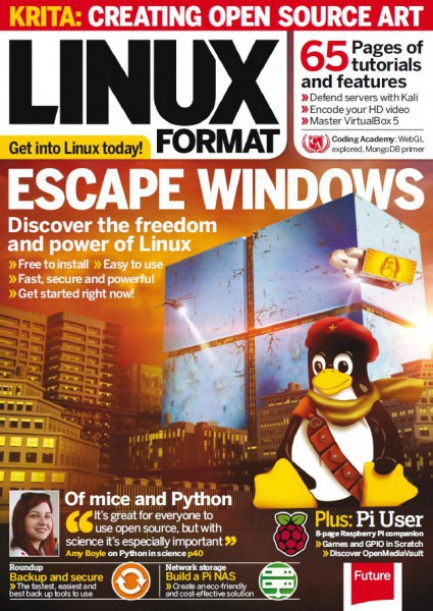
\includegraphics[height=5cm]{../pics/lf201602}
			\caption{\url{https://www.linuxformat.com}}
		\end{figure}
	\end{columns}
}

\end{document}

